\subsection{Generación de señalamiento paso a paso}

	Al ejecutar el RNA, primero detectará todos los \textit{netElements}, sus coordenadas iniciales y finales en la topología, y el sentido en el que fueron definidas. El resultado obtenido se muestra en el Cóodigo \ref{lst:EJ2_1}.
	
	\begin{lstlisting}[language = {}, caption = Detección de \textit{netElements} por parte del RNA , label = {lst:EJ2_1}]
		###### Starting Railway Network Analyzer #####
		Reading .railML file
		Creating railML object
		Analysing railML object
		Analysing graph
		ne14 [-1521, 450] [-560, 450] >>
		ne15 [-1521, 300] [-560, 450] >>
		ne16 [-560, 450] [516, 450] >>
		ne17 [516, 450] [666, 300] >>
		ne18 [516, 450] [1521, 450] >>
		ne19 [666, 300] [28, 300] <<
		ne20 [666, 300] [1521, 300] >>
		The network is connected
	\end{lstlisting}

	Por ejemplo, el \textit{netElement} ne19 inicia en la coordenada (666;300) y finaliza en la coordenada (28;300). El símbolo $<<$ indica que ne19 se encuentra definido de derecha a izquierda , ya que la componente x de la coordenada final es menor a la de la coordenada inicial, teniendo la misma componente y. Además, se puede comprobar que la lista obtenida en consistente con la Figura \ref{fig:EJ2_2}. Por ejemplo, ne14, ne15 y ne16 comparten la coordenada (-560,450), que coincide con la coordenada del cambio de vías Sw01.
	
	A continuación, el RNA detectará la infraestructura ferroviaria, las curvas peligrosas y los puntos medios de los netElements que el RNA considera demasiado largos. El resultado de este proceso se puede visualizar en el Código \ref{lst:EJ2_2} y puede leerse también en el archivo Infrastructure.RNA.
	
	\begin{lstlisting}[language = {}, caption = Detección de puntos críticos por parte del RNA , label = {lst:EJ2_2}]
		Analysing infrastructure --> Infrastructure.RNA
		Detecting Danger --> Safe_points.RNA
		ne14 has a Platform[plf116] @ [-1075, -450]
		ne15 has a Curve(2 lines) @ [[-710, 300]]
		ne16 has a LevelCrossing[lcr120] @ [-192, -450]
		ne18 has a Platform[plf117] @ [1111, -450]
		ne19 has a Middle point @ [347.0, 300]
		ne20 has a Middle point @ [1093.5, 300]
	\end{lstlisting}

	Una vez que el RNA detectó cada punto crítico de la red ferroviaria, procede a generar el señalamiento. El orden de generación no es importante, pero para poder describirlo de forma consistente se iniciará generando el señalamiento para proteger los finales de vías, las junturas entre rieles, las plataformas, los cruces de vía y los cambios de vías. Luego se procederá a mostrar el señalamiento pre y post simplificación. Las señales generadas para proteger los finales de vías relativos y absolutos son ilustradas en la Figura \ref{fig:EJ1_3}.

	\begin{figure}[H]
		\centering
		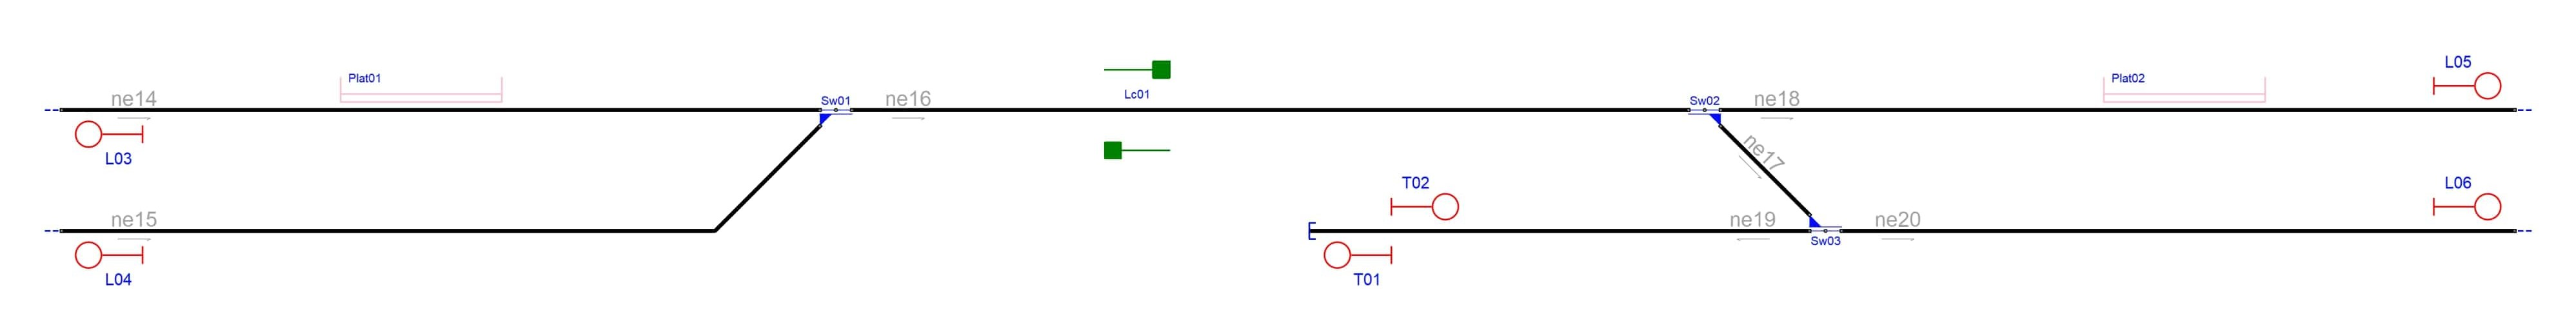
\includegraphics[width=1\textwidth]{resultados-obtenidos/ejemplo2/images/2_step1.png}
		\centering\caption{Señalamiento generado por el RNA para proteger el fín de vía.}
		\label{fig:EJ2_3}
	\end{figure}


	% ACA







\lipsum[1]

\begin{figure}[H]
	\centering
	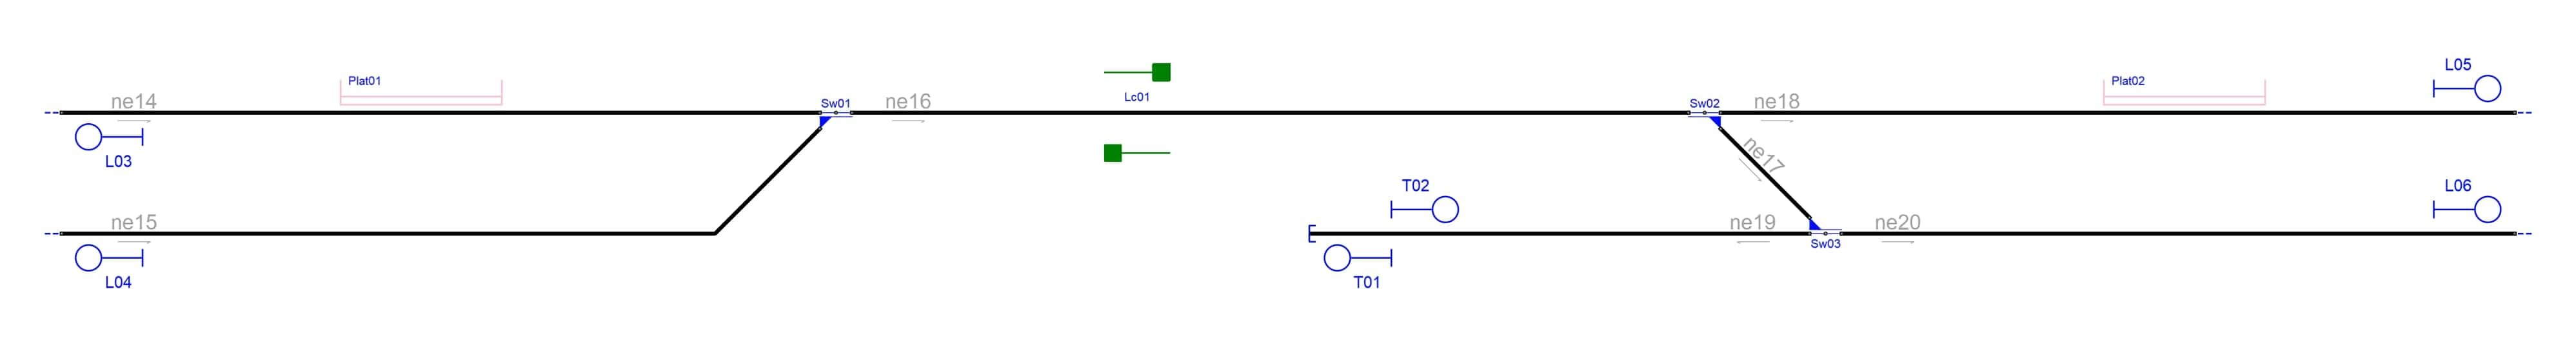
\includegraphics[width=1\textwidth]{resultados-obtenidos/ejemplo2/images/2_step2.png}
	\centering\caption{Señalamiento generado por el RNA para proteger las junturas.}
	%\label{fig:LC_P2}
\end{figure}

\lipsum[1]

\begin{figure}[H]
	\centering
	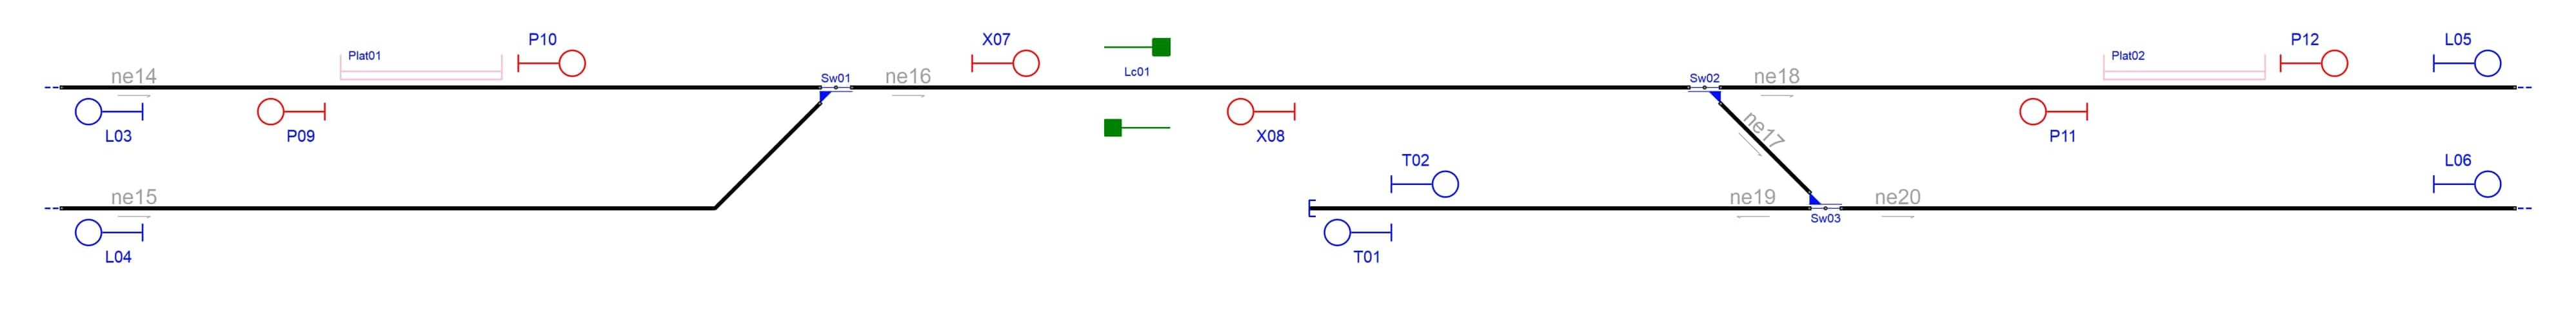
\includegraphics[width=1\textwidth]{resultados-obtenidos/ejemplo2/images/2_step3.png}
	\centering\caption{Señalamiento generado por el RNA para proteger plataformas y cruces de vía.}
	%\label{fig:LC_P2}
\end{figure}

\lipsum[1]

 \begin{figure}[H]
	\centering
	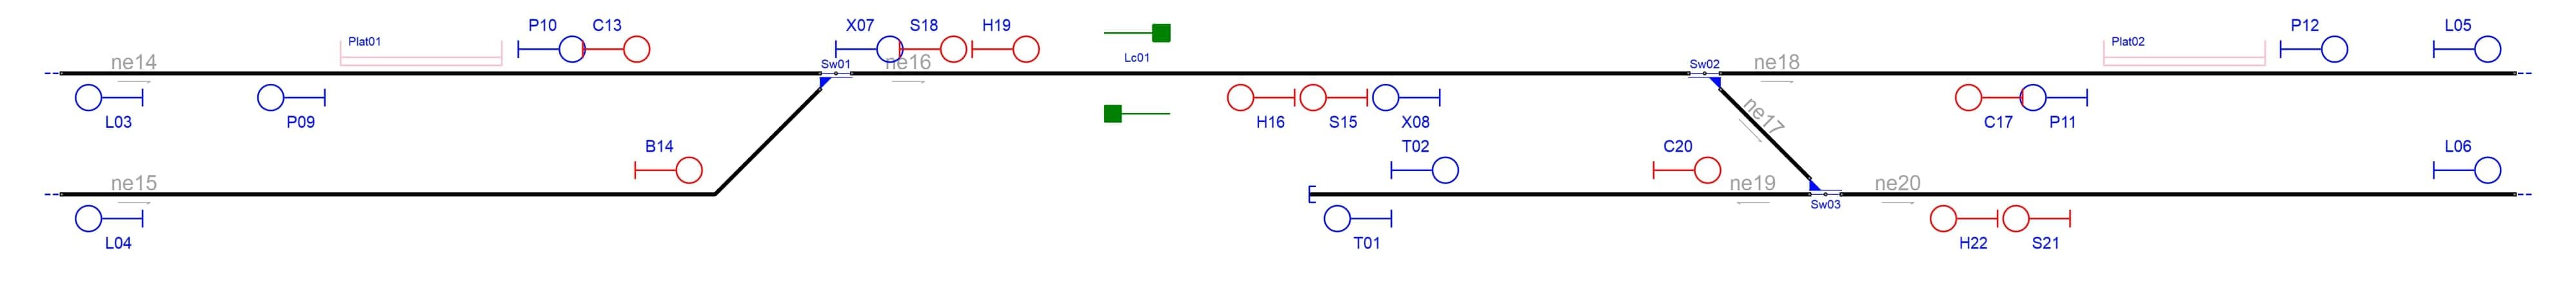
\includegraphics[width=1\textwidth]{resultados-obtenidos/ejemplo2/images/2_step4.png}
	\centering\caption{Señalamiento generado por el RNA para proteger las máquinas de cambios.}
	%\label{fig:LC_P2}
\end{figure}

\lipsum[1]

 \begin{figure}[H]
	\centering
	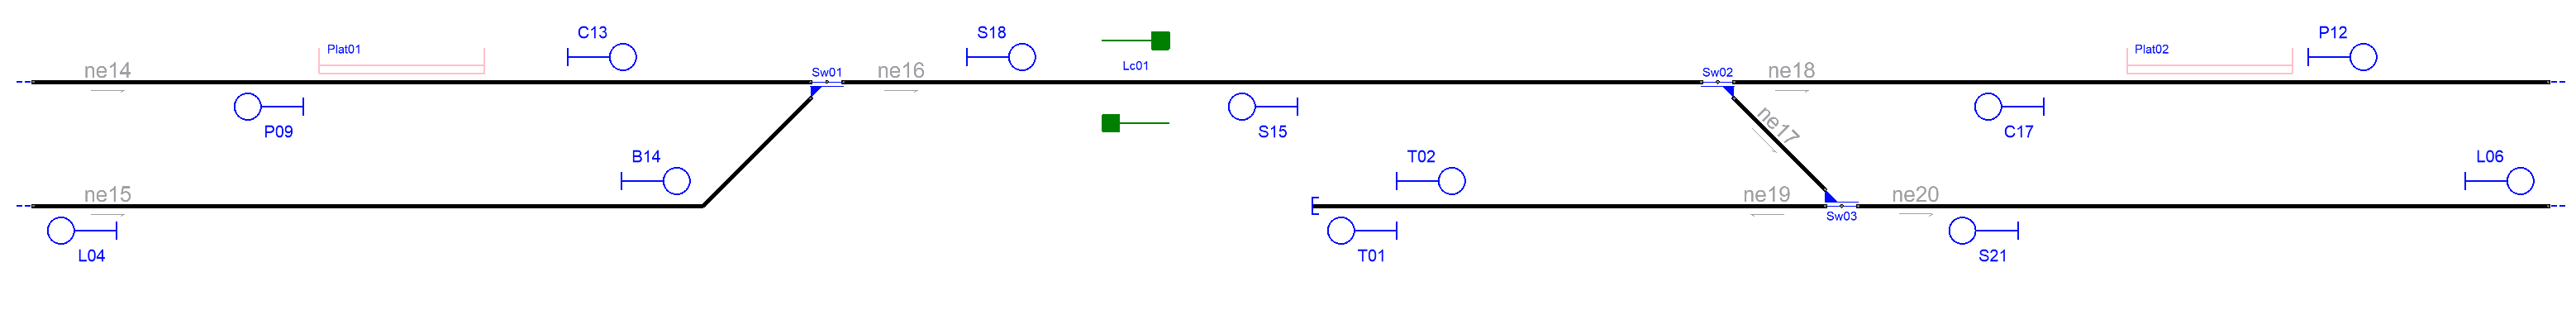
\includegraphics[width=1\textwidth]{resultados-obtenidos/ejemplo2/images/2_RNA.png}
	\centering\caption{Señalamiento generado y simplificado por el RNA.}
	%\label{fig:LC_P2}
\end{figure}

\lipsum[1]